\begin{frame}{Python on RPi}
	\begin{itemize}
		\item Used to program to access pins and process
		\item Can use any language!
		\item $C$ and $C++$ requires a compiler called \textbf{gcc} which is pre-installed
		\item Python interpreter is also pre-installed
		\item We shall use Python $3$ instead of Python $2$ here because most packages for RPi usage are written in Python $3$
	\end{itemize}
\end{frame}

\begin{frame}{Writing python code}
	\begin{itemize}
		\item Python programming Environments
		\begin{itemize}
			\item IDE
			\begin{itemize}
				\item Combines the facilities of interpreter and text editor
				\item Default IDE is IDLE
				\item Invoke: Menu $\rightarrow$ Programming $\rightarrow$ Python
				\item Select Python $3$
			\end{itemize}
			\item Text-editor and interpreter separately
			\begin{itemize}
				\item Use \textbf{nano} to write code (ex: hello.py)
				\item Execute the program by typing \textbf{python3 hello.py}
			\end{itemize}
		\end{itemize}
	\end{itemize}
\end{frame}

\begin{frame}{GPIO configuration}
	\begin{figure}
		\centering
		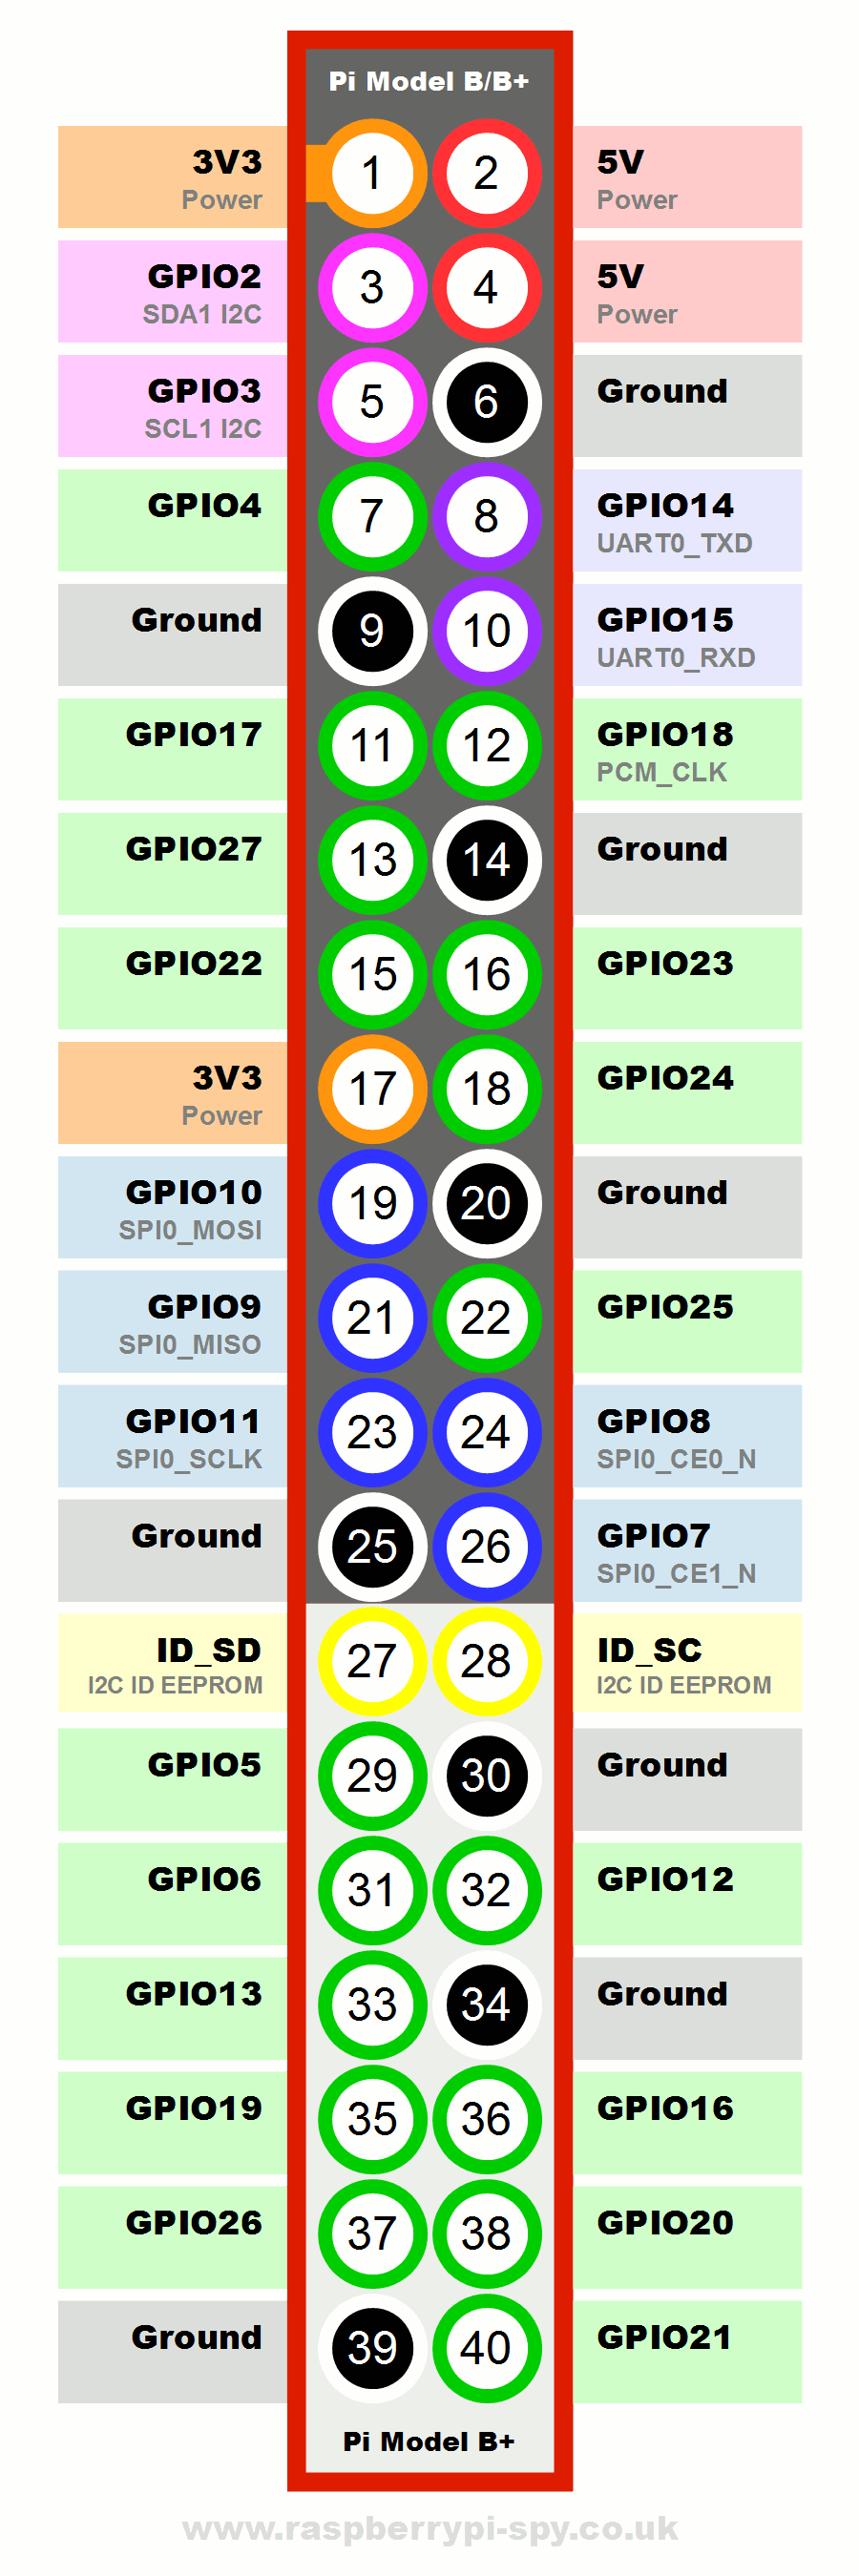
\includegraphics[width=4cm,height=7cm,keepaspectratio]{gpio}
	\end{figure}
\end{frame}

\begin{frame}{GPIO}
	\begin{itemize}
		\item Dedicated power and ground pins
		\begin{itemize}
			\item $3.3V (1,17)$
			\item $5V (2.4)$
			\item GND $(6,9,14,20,30,39)$
		\end{itemize}
		\item GPIO = General Purpose Input Output
		\item Make pins \textit{input} or \textit{output} pins as per choice
		\item There are two numbering systems
		\begin{itemize}
			\item pin number based on location
			\item Pin number given as GPIO1, GPIO2 etc.
		\end{itemize}
	\end{itemize}
\end{frame}

\begin{frame}{Protocol pins}
	\begin{itemize}
		\item \textbf{I2C}
		\begin{itemize}
			\item Pin no.3 (GPIO2) = SDA1 I2C
			\item Pin No.5 (GPIO3) = SCL1 I2C
			\item Serial communication protocol between two chips relatively closely placed and need to share a clock
			Two wire protocol (SDA = sends Data signal, SCL = sends Clock signal)
		\end{itemize}
		\item If there are several I2C compatible devices, one can connect their SDA and SCL lines together for serial communication between them
	\end{itemize}
\end{frame}

\begin{frame}{Protocol Pins}
	\begin{itemize}
		\item \textbf{SPI}
		\begin{itemize}
			\item 19 (GPIO10) = MOSI (Master Out Slave In)
			\item 21 (GPIO9) = MISO (Master In Slave Out)
			\item 23 (GPIO11) = SCLK (S Clock)
			\item 24 (GPIO8) = CE01 (Chip Enable)
			\item 26 (GPIO7) = CE02 (Chip Enable)
		\end{itemize}
	\end{itemize}
\end{frame}